\documentclass[10pt]{article}
\usepackage[utf8]{inputenc}
\usepackage{listings}
\usepackage{tabularx}
\usepackage{graphicx}
\usepackage{color}
\usepackage{alltt}
\usepackage[margin=1in]{geometry}
\usepackage{pdfpages}

\author{Rachel Hamilton, Jake Cousino}
\title{Amortization Table}
\date{Wednesday, June 20}
\definecolor{mygray}{gray}{0.6}


\lstset{
breaklines = true,
basicstyle=\footnotesize,
commentstyle=\color{green},
keywordstyle=\color{blue},
frame = triple,
numbers=left,
numbersep=5pt,
title = \lstname
}


\begin{document}
\maketitle
\tableofcontents
\vskip20mm
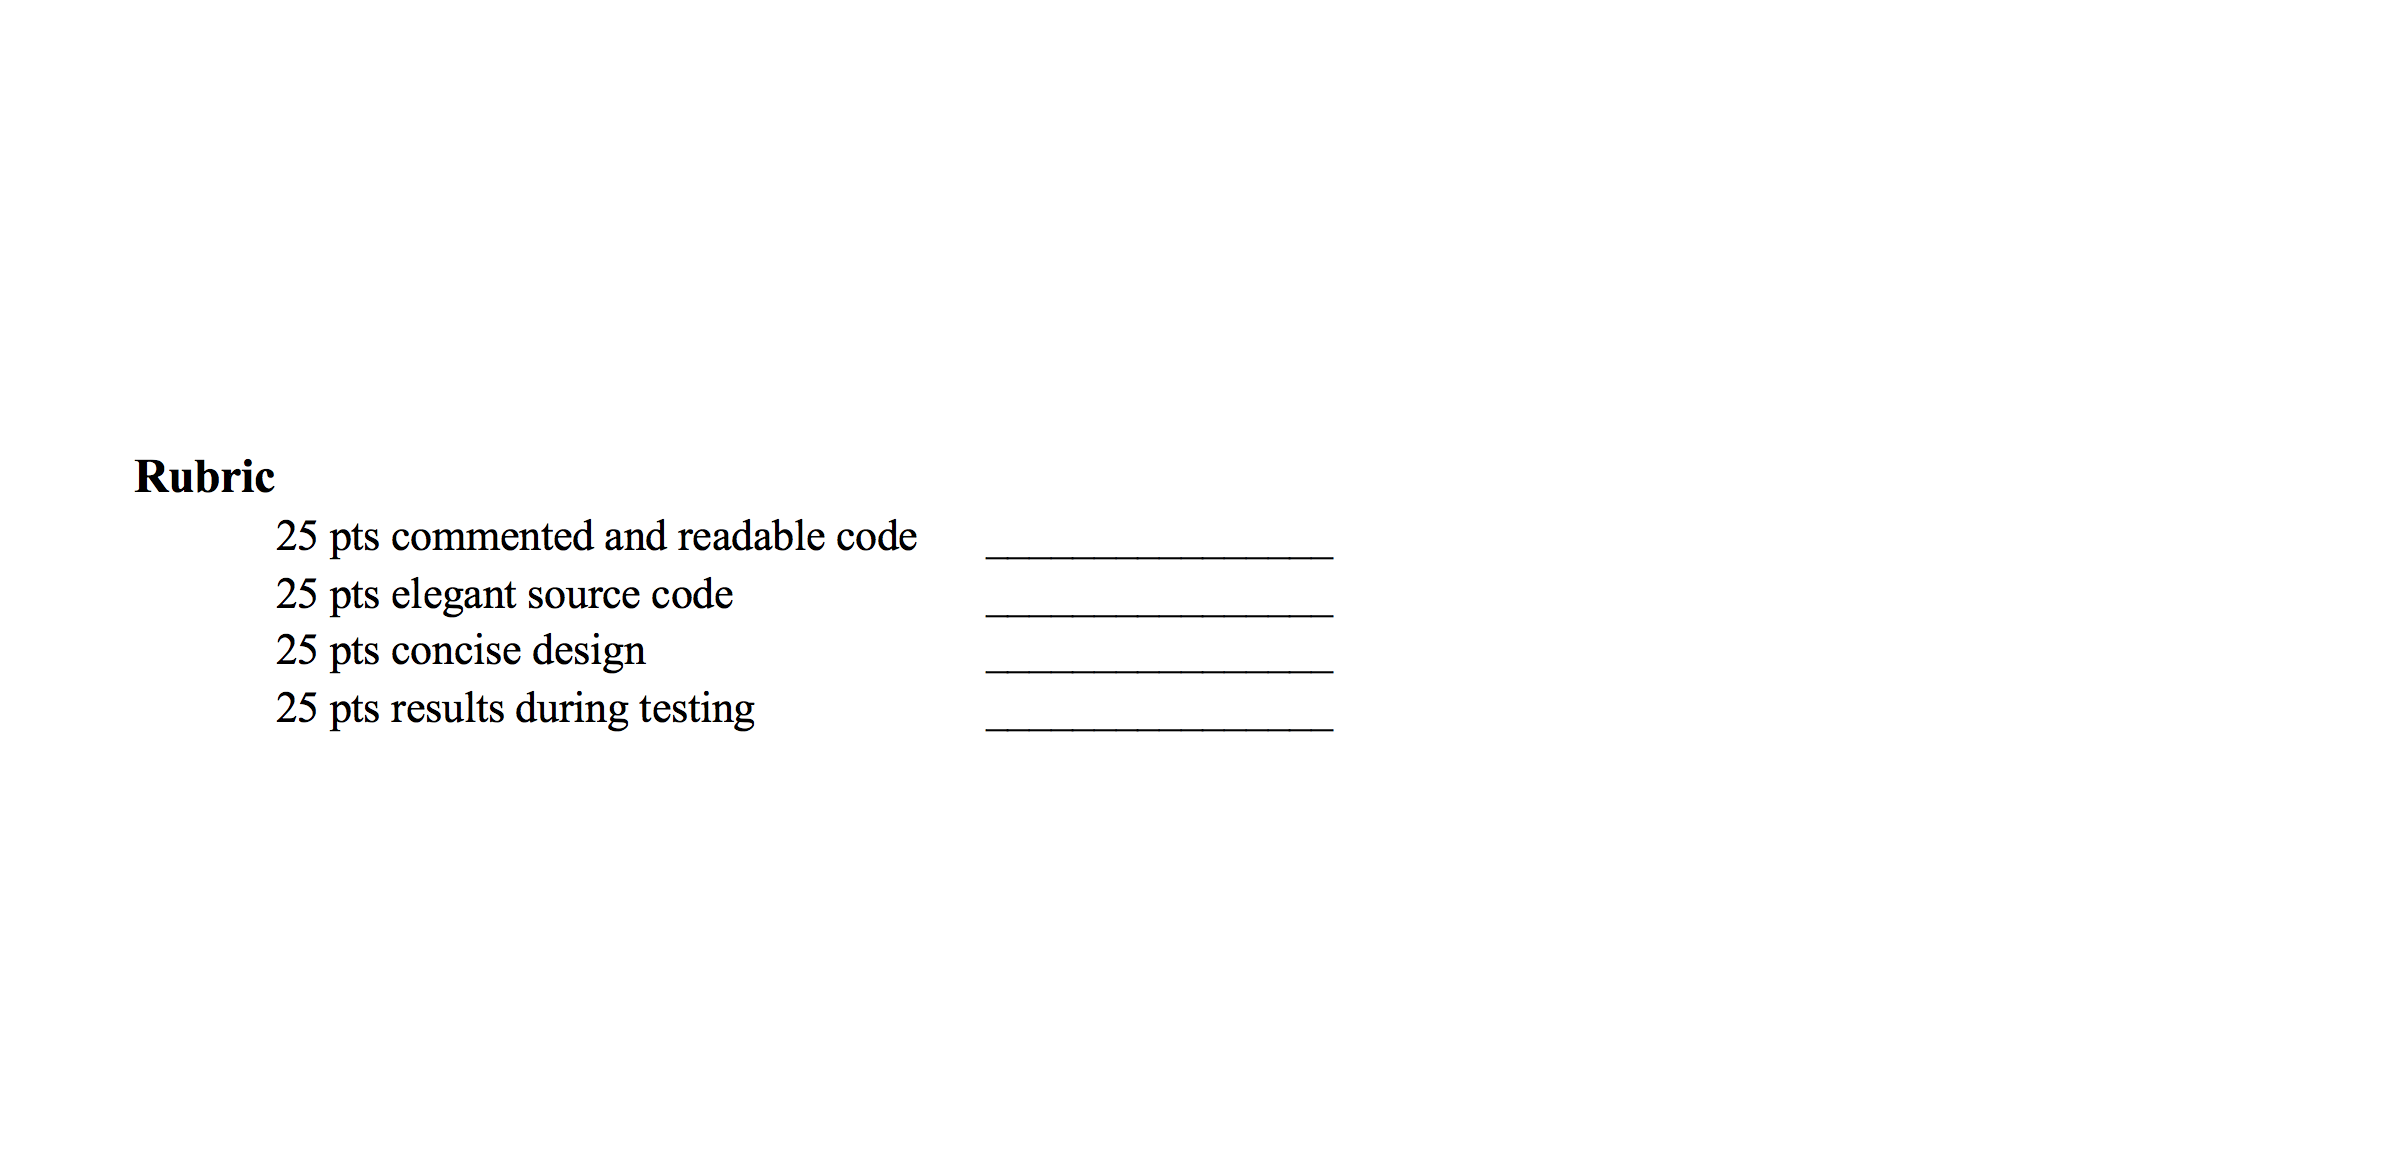
\includegraphics[width=\textwidth]{rubric.png}
\pagebreak
\part{Source Code}
\lstinputlisting[language=C++]{mazeSolver.cpp}
\pagebreak
\part{Output}
\begin{alltt}
\footnotesize
\input{MazeOutput.txt}
\end{alltt}
\end{document}
